\documentclass[a4paper]{article}

\usepackage[english]{babel}
\usepackage[utf8x]{inputenc}
\usepackage{amsmath}
\usepackage{graphicx}
\usepackage[colorinlistoftodos]{todonotes}
\title{Joint Modeling of Content-Partitioned Multinetwork Embeddings (CPME) and Point Process Approach}
\author{Bomin Kim}

\begin{document}
\maketitle

\begin{abstract}
Your abstract.
\end{abstract}

\section{Ideas}
Current CPME model does not involve any of temporal component, which plays a key role in email interactions. Intuitively, past interaction behaviors significantly influence future ones; for example, if an actor $i$ sent an email to actor $j$, then $j$ is highly likely to send an email back to $i$ as a response (i.e. reciprocity). Moreover, the recency and frequency of past interactions can also be considered to effectively predict future interactions. Thus, as an exploratory data analysis, point process model for directional interaction is applied to the North Carolina email data. Starting from the existing framework focused on the analysis of content-partitioned subnetworks, I would suggest an extended approach to analyze the data using the timestamps in the email, aiming to develop a joint dynamic or longitudinal model of text-valued ties.\\ \newline
 CPME model is a Bayesian framework using two well-known methods: Latent Dirichlet Allocation (LDA) and Latent Space Model (LSM). Basically, existence of edge depends on topic assignment t (LDA) and its corresponding interaction pattern c. Each topic t=1,…,T has one interaction pattern c=1,…,C, and each interaction pattern posits unique latent space (LSM), thus generating $A\times A$ matrix of probabilities $P^{(c)}$ that a message author
a will include recipient $r$ on the message, given that it is about
a topic in cluster $c$.  Incorporating point process approach, now assume that under each interaction pattern, we have $A\times A$ matrix of probabilities $P^{(c)}$ which not only depend on the latent space, but also on the history of interaction between the sender and receiver. 
\newpage
\section{Preliminary Analysis}
Hurricane Sandy was the most destructive hurricane in 2012, which hit North Carolina on late October (October 28, Governor Bev Perdue declared a state of emergency in 24 western counties due to snow and strong winds). In our dataset, there are three counties which cover the date of Hurricane Sandy (October 22, 2012 – November 2, 2012), so we focus on the three counties, since the timestamp of email in this case is much more important than usual case without any disastrous event.
\subsection{Dare County}
\footnotesize
\begin{table}[ht]
	\centering
	\begin{tabular}{ |c|ccc|c| } 
		\hline 
		\textbf{Period} &\textbf{Before Sandy} & \textbf{During Sandy} & \textbf{After Sandy} & \textbf{Overall} \\ 	\hline
			\textbf{\# emails}& 1933 & 1563 & 1467 & 4963 \\ 
		\hline
	\end{tabular}
	\caption{ Summary of Dare county email data based on time period}
	\label{table:nullDare2}
\end{table}
\normalsize
Before Sandy ranges from 2012-09-01 to 2012-10-21 (7 weeks), During Sandy ranges from 2012-10-22 to 2012-11-02 (2 weeks), and After Sandy ranges from 2012-11-03 to 2012-11-30 (4 weeks).
\footnotesize
\begin{figure}[ht]
	\centering
	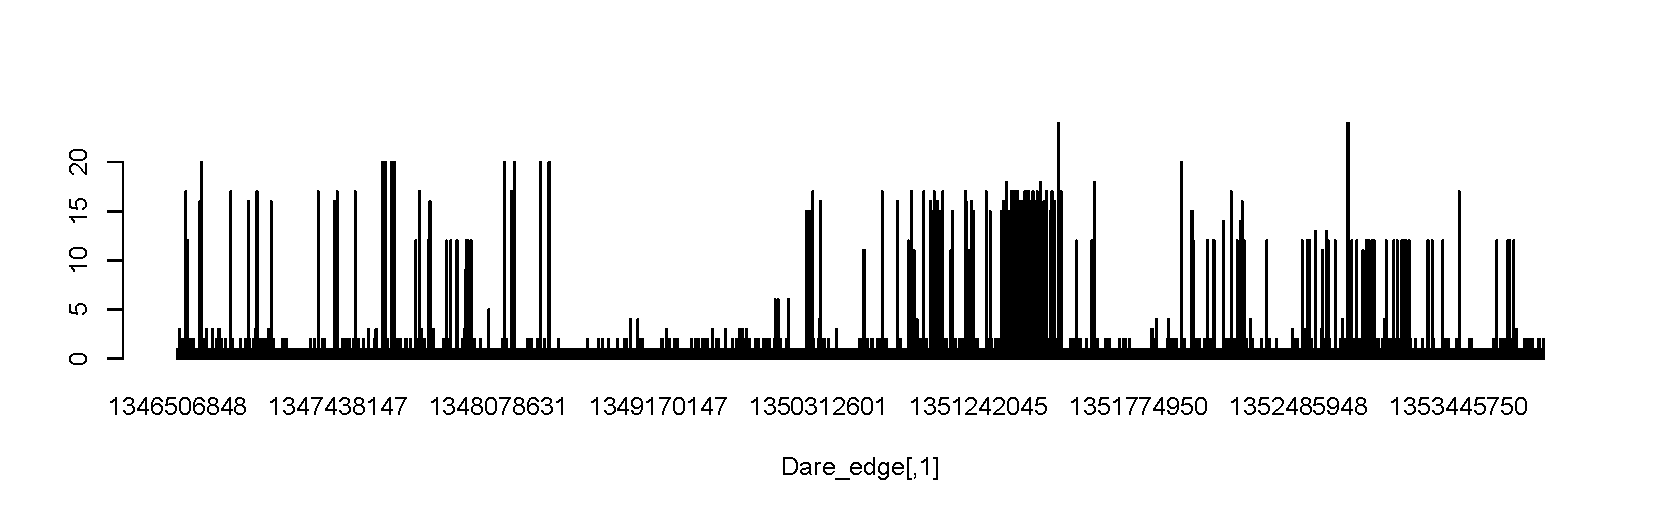
\includegraphics[width=1.1\textwidth]{DareEmails.pdf} 
	\caption{Frequency of Dare county emails from 2012-09-01 to 2012-11-30  }
	\label{fig:Emailplots}
\end{figure}
\begin{table}[ht]
	\centering
	\begin{tabular}{ |c|cc| } 
		\hline 
		\textbf{Time Interval} &\textbf{send} & \textbf{receive} \\ 	
		\hline  $[-\infty, t)$&  2.128, 2.659, 2.355, 2.919& 0.292, 0.257, 0.047, 0.110\\  $[t-30 m, t)$ &  0.262, -0.064, 0.782, 0.317 &2.087, 1.287 , 2.346, 1.870\\  $[t-2h, t-30m)$& 0.383, 0.157 , 0.024, -0.045 &0.553, 0.082, 0.794, 0.269\\ $[t-8h, t-2h)$ & 0.816, 0.054 , 0.077, 0.381 &-0.221, 0.048, 0.298, -0.012 \\ $[t-32h, t-8h)$& 0.085, 0.014,  0.228, 0.070 &0.101, 0.017, -0.033, 0.019\\ $[t-5.33d, t-32h)$&  0.103, 0.025, 0.092, 0.008 &-0.027, -0.016, -0.033, -0.009 \\ $[t-21.33d, t-5.33d)$  & 0.052, 0.000, 0.059, 0.010& 0.013, 0.030 , -0.016, 0.013\\ 
		$[-\infty, t-21.33d)$  & 0.052, 0.103, 0.027, 0.021  & 0.008, 0.000, 0.020, -0.005\\
		\hline
	\end{tabular}
	\caption {Estimated coefficients and approximate standard errors for dyadic effects of Dare county data (before Sandy, during Sandy, after Sandy, overall)}
	\label{table:nullDare}
\end{table}
\footnotesize
\begin{figure}[ht]
	\centering
	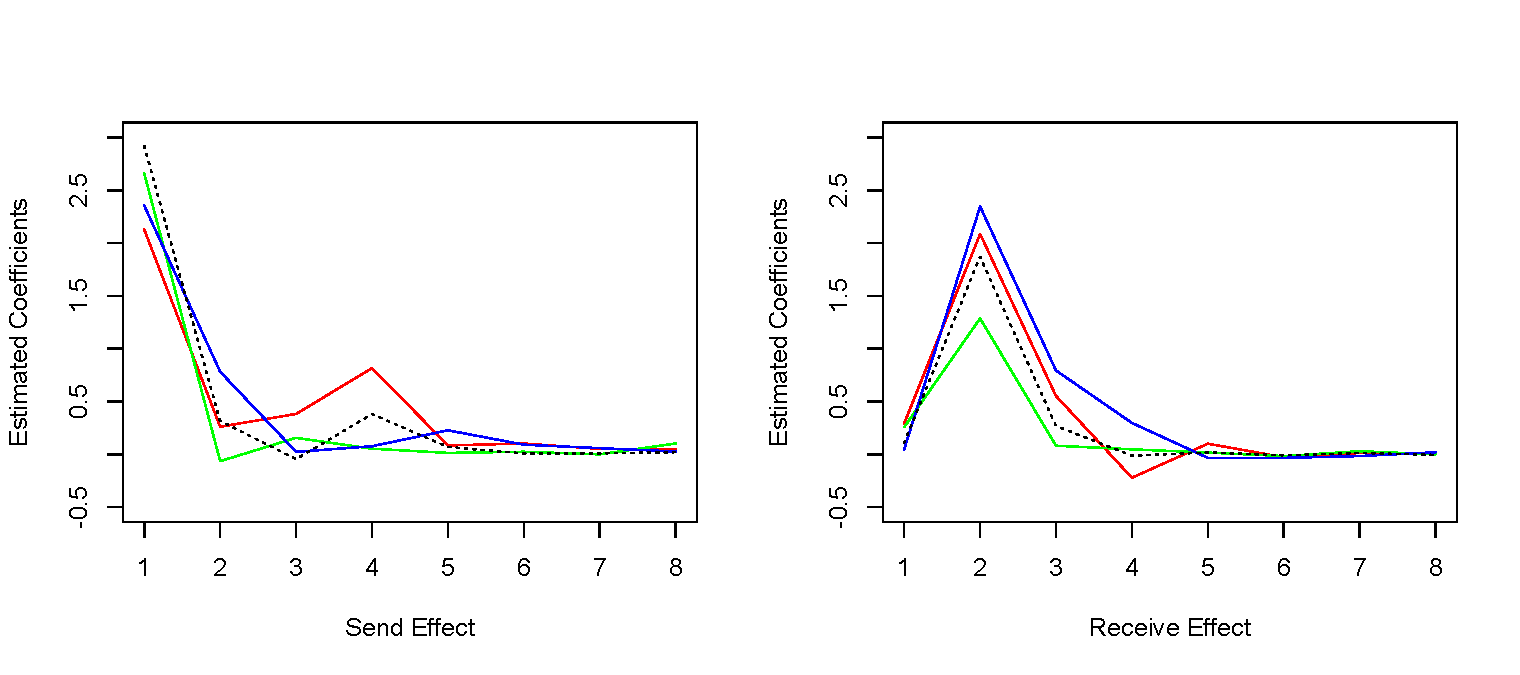
\includegraphics[width=1.1\textwidth]{Dareplot.pdf} 
	\caption{Comparison of Send (left) and Receive (right) effect based on periods in Table 1. (Red=Before, Green=During, Blue=After, and dot=Overall)}	\label{fig:Emailplot}
\end{figure}
\subsection{Lenoir County}
\footnotesize
\begin{table}[ht]
	\centering
	\begin{tabular}{ |c|ccc|c| } 
		\hline 
		\textbf{Period} &\textbf{Before Sandy} & \textbf{During Sandy} & \textbf{After Sandy} & \textbf{Overall} \\ 	\hline
		\textbf{\# emails}& 216 & 83 & 302 & 601 \\ 
		\hline
	\end{tabular}
	\caption{ Summary of Lenoir county email data based on time period}
	\label{table:nullDare2}
\end{table}
\normalsize
Before Sandy ranges from 2012-10-01 to 2012-10-21 (3 weeks), During Sandy ranges from 2012-10-22 to 2012-11-02 (2 weeks), and After Sandy ranges from 2012-11-03 to 2012-12-31 (8 weeks).
\footnotesize
\begin{figure}[ht]
	\centering
	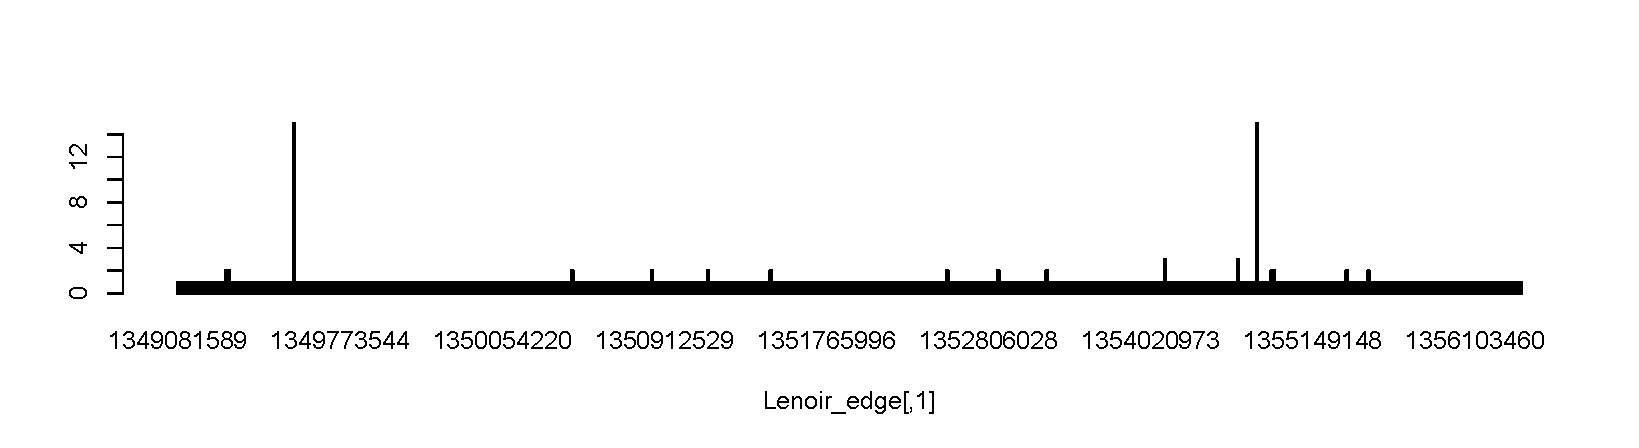
\includegraphics[width=1.1\textwidth]{LenoirEmails.pdf} 
	\caption{Frequency of Lenoir county emails from 2012-10-01 to 2012-12-31  }
	\label{fig:Emailplots2}
\end{figure}
\newpage
\subsection{Vance County}
\footnotesize
\footnotesize
\begin{table}[ht]
	\centering
	\begin{tabular}{ |c|ccc|c| } 
		\hline 
		\textbf{Period} &\textbf{Before Sandy} & \textbf{During Sandy} & \textbf{After Sandy} & \textbf{Overall} \\ 	\hline
		\textbf{\# emails}& 198& 18 & 55 & 271 \\ 
		\hline
	\end{tabular}
	\caption{ Summary of Vance county email data based on time period}
	\label{table:nullVance}
\end{table}
\normalsize
Before Sandy ranges from 2012-09-04 to 2012-10-21 (7 weeks), During Sandy ranges from 2012-10-22 to 2012-11-02 (2 weeks), and After Sandy ranges from 2012-11-03 to 2012-11-30  (4 weeks).
\footnotesize
\begin{figure}[ht]
	\centering
	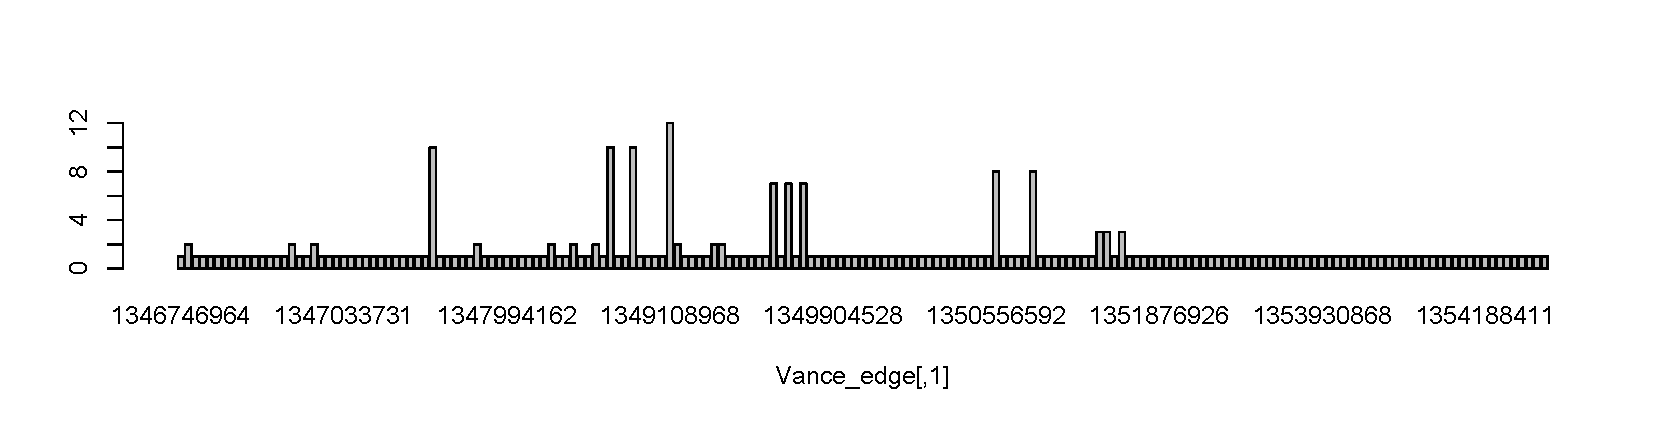
\includegraphics[width=1.1\textwidth]{VanceEmails.pdf} 
	\caption{Frequency of Vance county emails from 2012-09-04 to 2012-11-30  }
	\label{fig:Emailplots2}
\end{figure}
\end{document}